\chapter{HLS Pragmas and Approximations}

The previous chapters have defined the algorithm. This chapter focuses on the \textbf{hardware implementation} of primarly the HLS aspects of ViT. \textbf{High Level Synthesis(HLS)} is the process of converting the high-level C/C++ code into a \textbf{Hardware circuit} without the need for writing Veriolog or RTL code manually.

\section{What is High-Level Synthesis (HLS)?}

High-Level Synthesis (HLS) is a design methodology that translates  high-level language C/C++ code into a low-level hardware description (RTL, or Register-Transfer Level) that can be implemented on an FPGA \cite{ref5, ref6}.

The primary goal of HLS is to bridge the "productivity gap." Manually writing RTL (in VHDL or Verilog) is extremely time-consuming and error-prone, especially for complex algorithms like neural networks. HLS allows the designer to focus on the \textit{algorithm} and \textit{architecture} rather than low-level, cycle-by-cycle hardware implementation \cite{ref6}.

Some Leading FPGA vendors also provide sophisticated HLS Software/tools, such as the \textbf{AMD Vitis HLS} platform used for this project \cite{ref6}. These tools have rich features to parse C++ code, but might require explicit guidance to  create an efficient design.

\section{The Role of HLS Pragmas}

By default, the HLS compiler will create a hardware implementation that is \textbf{functionally correct} but \textbf{slow}. It will synthesize loops to run sequentially, one iteration after another, and might store arrays in large, single-port memories, which are very inefficient to read and write. This "default" hardware is resource-efficient but has terrible performance.

To create a high-performance accelerator, the designer must explicitly \textit{guide} the HLS tool on how to build the hardware. This is done using compiler directives called \textbf{pragmas} \cite{ref2}.

Pragmas can exactly pin-point where to store arrays and how to unroll loops. They are inserted as comments (\texttt{\#pragma HLS...}) into the C++ source code. They allow the designer to control the core trade-off of hardware design: \textbf{performance vs. area} (i.e., latency and throughput vs. FPGA resource utilization \cite{ref3}).

The HLS code for this ViT accelerator uses a very rich set of pragmas to build a highly parallel and pipelined architecture. Here are some of the important HLS pragmas used in ViT implementation.

\section{Loop Optimization Pragmas}

These are the most critical pragmas for achieving high performance. They transform sequential loops into parallel hardware.

\subsection{\texttt{\#pragma HLS PIPELINE II=1}}
This is one of the most important pragma for throughput. It instructs HLS to \textbf{pipeline} the execution of a loop \cite{ref7}.
\begin{itemize}
    \item \textbf{Without Pipelining:} A loop that takes 5 clock cycles per iteration will take 500 cycles for 100 iterations.
    \item \textbf{With Pipelining:} The loop's operations are overlapped, similar to assembly language. While Iteration 1 is in its 5th cycle, Iteration 2 is in its 4th, Iteration 3 in its 3rd, and so on \cite{ref7}.
    \item \textbf{II=1:} The \texttt{II} stands for "Initiation Interval." An \texttt{II=1} means the pipeline can and start a new loop iteration \textbf{every single clock cycle} \cite{ref9, ref10}.
\end{itemize}
With II=1, the loop that took \textbf{500} cycles earlier, can now be completed in just \textbf{104} cycles, achieving massive speedup (i.e 5x). This pragma is used in almost every critical loop of my ViT implementation (e.g., \texttt{QKV\_ACC\_I}, \texttt{SCORES\_J}, \texttt{ADD\_MLP\_J}).



\subsection{\texttt{\#pragma HLS UNROLL}}
This pragma achieves parallelism by \textbf{duplicating hardware}. It "unrolls" a loop, creating physical, parallel copies of the loop body's hardware \cite{ref10, ref13}.
\begin{itemize}
    \item \textbf{Example:} A loop that calculates sum of 16 numbers. By default, the hardware would consist of only one adder and would take 16 cycles to complete..
    \item \textbf{\texttt{factor=16}:} With \texttt{UNROLL factor=16}, HLS will provides \textbf{16 physical adders} to perform all 16 additions in a single clock cycle. This reduces latency drastically but will consume more hardware resources \cite{ref15, ref16}.
\end{itemize}
This loop unroll pragma is used in the \texttt{patch\_to\_embed\_from\_img} function (\texttt{factor=16}) to parallelize the dot product, and in \texttt{mha\_block} (\texttt{factor=4}) to parallelize parts of the attention calculation.

\subsection{\texttt{\#pragma HLS LOOP\_MERGE}}
This pragma instructs HLS to merge two or more \textit{consecutive} smaller loops  into a single, larger loop.
\begin{itemize}
    \item \textbf{Benefit:} Merging loops reduces the overhead of transitioning between them (the exit and entry logic).
\end{itemize}

\section{Memory and Resource Pragmas}

\subsection{\texttt{\#pragma HLS ARRAY\_PARTITION}}
This pragma is the generally used along with loop \texttt{UNROLL} and \texttt{PIPELINE}. It solves the memory bottleneck that parallel hardware creates \cite{ref12}.
\begin{itemize}
    \item \textbf{Bottleneck:} A standard array is stored in a Block RAM (BRAM), which has only one or two "ports" (allowing 1-2 reads/writes per cycle). If you \texttt{UNROLL} a loop by 16 factor, then all the 16 adders  try to read from the \textit{same} BRAM at the same time. They will stall, and the \texttt{II=1} pipeline will fail \cite{ref13}.
    \item \textbf{Solution:} \texttt{ARRAY\_PARTITION} physically splits the single large array into multiple smaller, independent arrays (or registers) typically into different BRAM cells, where each cell has its own read and write port \cite{ref18, ref19}.
\end{itemize}
The syntax is \texttt{\#pragma HLS ARRAY\_PARTITION variable=<A> <TYPE> factor=<N> dim=<D>}. The \texttt{TYPE} here specifies the type of partition:
\begin{itemize}
    \item \textbf{\texttt{complete}:} This type partitions  the array completely, implementing every single element as a separate register. This provides maximum parallelism but uses more number of resources. Typically used for smaller arrays which are accessed with very high frequency
    \item \textbf{\texttt{block}:} This splits the array into \texttt{N} contiguous blocks. For example, \texttt{factor=4} on an array of 16 elements would create four new arrays: `[0-3]`, `[4-7]`, `[8-11]`, and `[12-15]`.
    \item \textbf{\texttt{cyclic}:} This splits the array into \texttt{N} interleaved smaller arrays.For example, with factor = 4 on 16 elements, the elements are distributed cyclically across 4 banks:
    \begin{itemize}
        \item \textbf{Bank 0}: [0, 4, 8, 12]
        \item \textbf{Bank 1}: [1, 5, 9, 13]
        \item \textbf{Bank 2}: [2, 6, 10, 14]
        \item \textbf{Bank 3}: [3, 7, 11, 15]
    \end{itemize}
    This is the most powerful type for pipelined loops. In my code (\texttt{layer\_norm}), \texttt{cyclic factor=16} ensures that 16 consecutive loop iterations (i, i+1,... i+15) access 16 different physical memories, enabling simultaneous access and a true \texttt{II=1} pipeline.
\end{itemize}

\subsection{\texttt{\#pragma HLS BIND\_STORAGE}}
This pragma gives explicit control over the \textit{type} of memory used for an array \cite. While \texttt{ARRAY\_PARTITION} splits an array, \texttt{BIND\_STORAGE} decides what kind of array to map it to.
\begin{itemize}
    \item \textbf{\texttt{type=ram\_2p impl=bram}:} This directive, used heavily in \texttt{mha\_block}, tells HLS: "Implement this array (e.g., \texttt{Q}, \texttt{K}, \texttt{V}) using a dual-port RAM (\texttt{ram\_2p}) and specifically use the FPGA's built-in \textbf{Block RAM (BRAM)} resources (\texttt{impl=bram})".
    \item \textbf{\texttt{type=ram\_4p impl=uram}:} An alternative is to use \textbf{Ultra RAM }for arrays which use more memory. One BRAM cell is generally of 10-20 KB, so URAM would be use in case of higher memory footprint.
\end{itemize}

\section{Interface and Task-Level Pragmas}

\subsection{\texttt{\#pragma HLS INTERFACE}}
This pragma is one of the most important, as it defines the external ports of the accelerator—how it connects to the rest of the system. It is only used on the arguments of the top-level function (\texttt{vit\_top}).
\begin{itemize}
    \item \textbf{\texttt{s\_axilite}:} Creates a "slave" AXI-Lite interface. This is a simple, low-bandwidth port used for control registers. The host CPU uses this to send scalar values (like configuration data) and to start/stop/check the accelerator.
    \item \textbf{\texttt{m\_axi}:} Creates a "master" AXI interface. This is a high-performance, high-bandwidth port that allows the accelerator to read and write directly to global memory (DRAM). This is essential for large data buffers like the input image (\texttt{img}) and the final \texttt{out\_logits}.
\end{itemize}

% \subsection{\texttt{\#pragma HLS DATAFLOW}}
% This pragma enables \textit{task-level parallelism}. Instead of just pipelining loops (fine-grained parallelism), \texttt{DATAFLOW} pipelines entire functions (coarse-grained parallelism).
% \begin{itemize}
%     \item \textbf{Operation:} When applied to a region of code, HLS attempts to execute each function call in that region as a separate, concurrent hardware process. These processes communicate with each other using internal "streaming" FIFO buffers.
%     \item \textbf{Example:} A common pattern is \texttt{read\_data()}, \texttt{compute\_data()}, \texttt{write\_data()}. With \texttt{DATAFLOW}, the \texttt{compute\_data} function can start working on the first block of data as soon as \texttt{read\_data} passes it, while \texttt{read\_data} simultaneously fetches the *next* block of data.
% \end{itemize}

\subsection{\texttt{\#pragma HLS INLINE}}
This pragma is a "logic" pragma. When applied to a function, it tells HLS not to create a separate, self-contained hardware module for that function. Instead, it "inlines" the function's logic directly into the calling function.
\begin{itemize}
    \item \textbf{Benefit:} This removes the latency and overhead of a hardware-level function call (which involves handshaking signals).
    \item \textbf{Usage:} It is mainly used for small, helper functions like \texttt{layer\_norm}, \texttt{make\_prune\_mask}, and \texttt{softmax\_seq} so that their logic is directly absorbed into the main \texttt{transformer\_block} and \texttt{mha\_block} pipelines.
\end{itemize}
\begin{table}[H]
\centering
    \renewcommand{\arraystretch}{1.25}
    \begin{tabularx}{\textwidth}{|>{\raggedright\arraybackslash}p{2.8cm}|>{\raggedright\arraybackslash}p{4cm}|>{\raggedright\arraybackslash}X|}
        \hline
        \textbf{Pragma} & \textbf{Purpose} & \textbf{Example in Code} \\
        \hline
        \texttt{INTERFACE} & Defines external ports for control (s\_axilite) and memory (m\_axi). & \texttt{vit\_top} arguments (\texttt{img}, \texttt{out\_logits}) \\
        \hline
        \texttt{PIPELINE II=1} & Enables processing one loop iteration per cycle. & \texttt{QKV\_ACC\_I}, \texttt{SCORES\_J}, \texttt{WRITE\_HEAD} \\
        \hline
        \texttt{UNROLL} & Creates parallel hardware for loop iterations. & \texttt{patch\_to\_embed\_from\_img (factor=16)} \\
        \hline
        % \texttt{LOOP\_FLATTEN} & Merges nested loops into one. (\texttt{off} prevents this). & \texttt{PATCH\_ROWS} loop (\texttt{off} is used) \\
        % \hline
        % \texttt{DATAFLOW} & Executes functions concurrently (task-level pipeline). & (Conceptual: used for pipelining `read-compute-write` blocks) \\
        \hline
        \texttt{ARRAY\_PARTITION} & Splits arrays for parallel memory access. & \texttt{seq}, \texttt{ln1\_out (cyclic factor=16)} \\
        \hline
        \texttt{BIND\_STORAGE} & Forces an array into a specific memory type (BRAM). & \texttt{Q}, \texttt{K}, \texttt{V (type=ram\_2p impl=bram)} \\
        \hline
        \texttt{INLINE} & Folds a function's logic into its caller. & \texttt{layer\_norm}, \texttt{make\_prune\_mask} \\
        \hline
    \end{tabularx}
    \caption{Summary of key HLS pragmas used in the ViT accelerator.}
    \label{table:pragma_summary}
\end{table}

\section{The Synthesizability Gap: Software vs. Hardware}

In a standard C++ environment, functions like \texttt{expf()}, \texttt{tanhf()}, \texttt{sqrtf()}, and \texttt{erf()} are provided by the \texttt{math.h} library. These are complex, software-based routines that may use iterative algorithms, look-up tables for computing results.

The Vitis HLS compiler cannot synthesize these functions. HLS is designed to create a \textit{static, deterministic hardware circuit}—a collection of logic gates, adders, and multipliers. It does not know how to build a hardware circuit for a complex, iterative software function.
Therefore, every "non-synthesizable" function must be replaced with a "hardware-friendly" equivalent. This is achieved in two ways:
\begin{enumerate}
    \item \textbf{Using the HLS Math Library:} AMD provides a specific library, \texttt{hls\_math.h}, which contains synthesizable, hardware-optimized versions of these functions (e.g., \texttt{hls::expf}, \texttt{hls::sqrtf}) \cite{ref12}.
    \item \textbf{Manual Approximation:} For some functions, which are not present in any libary, it is advised to manually implement a well-known mathematical approximation \cite{ref4, ref5}.
\end{enumerate}

\section{Approximating the GELU Activation Function}

The standard activation function in any Transformer architecture is the Gaussian Error Linear Unit (GELU). Its mathematical definition depends on Gaussian Error Function, \texttt{erf}:

\[
\text{GELU}(x) = 0.5 \cdot x \cdot \left( 1 + \text{erf}\left(\frac{x}{\sqrt{2}}\right) \right)
\]

The \texttt{erf} function is complex and non-synthesizable \cite{ref5}. To solve this, we used a highly accurate approximation that replaces the \texttt{erf} portion with a function based on (\texttt{tanh}) \cite{ref6}.
\begin{verbatim}
static inline float gelu(float x) {
    return 0.5f * x * (1.0f + tanhf(0.79788456f *
        (x + 0.044715f * x * x * x)));
}
\end{verbatim}

It replaces the non-synthesizable \texttt{erf} with some basic arithmetic (add, multiply) and the \texttt{tanhf} function, which can itself be synthesized by including the \texttt{hls\_math.h} library.

\begin{figure}[h!]
    \centering
    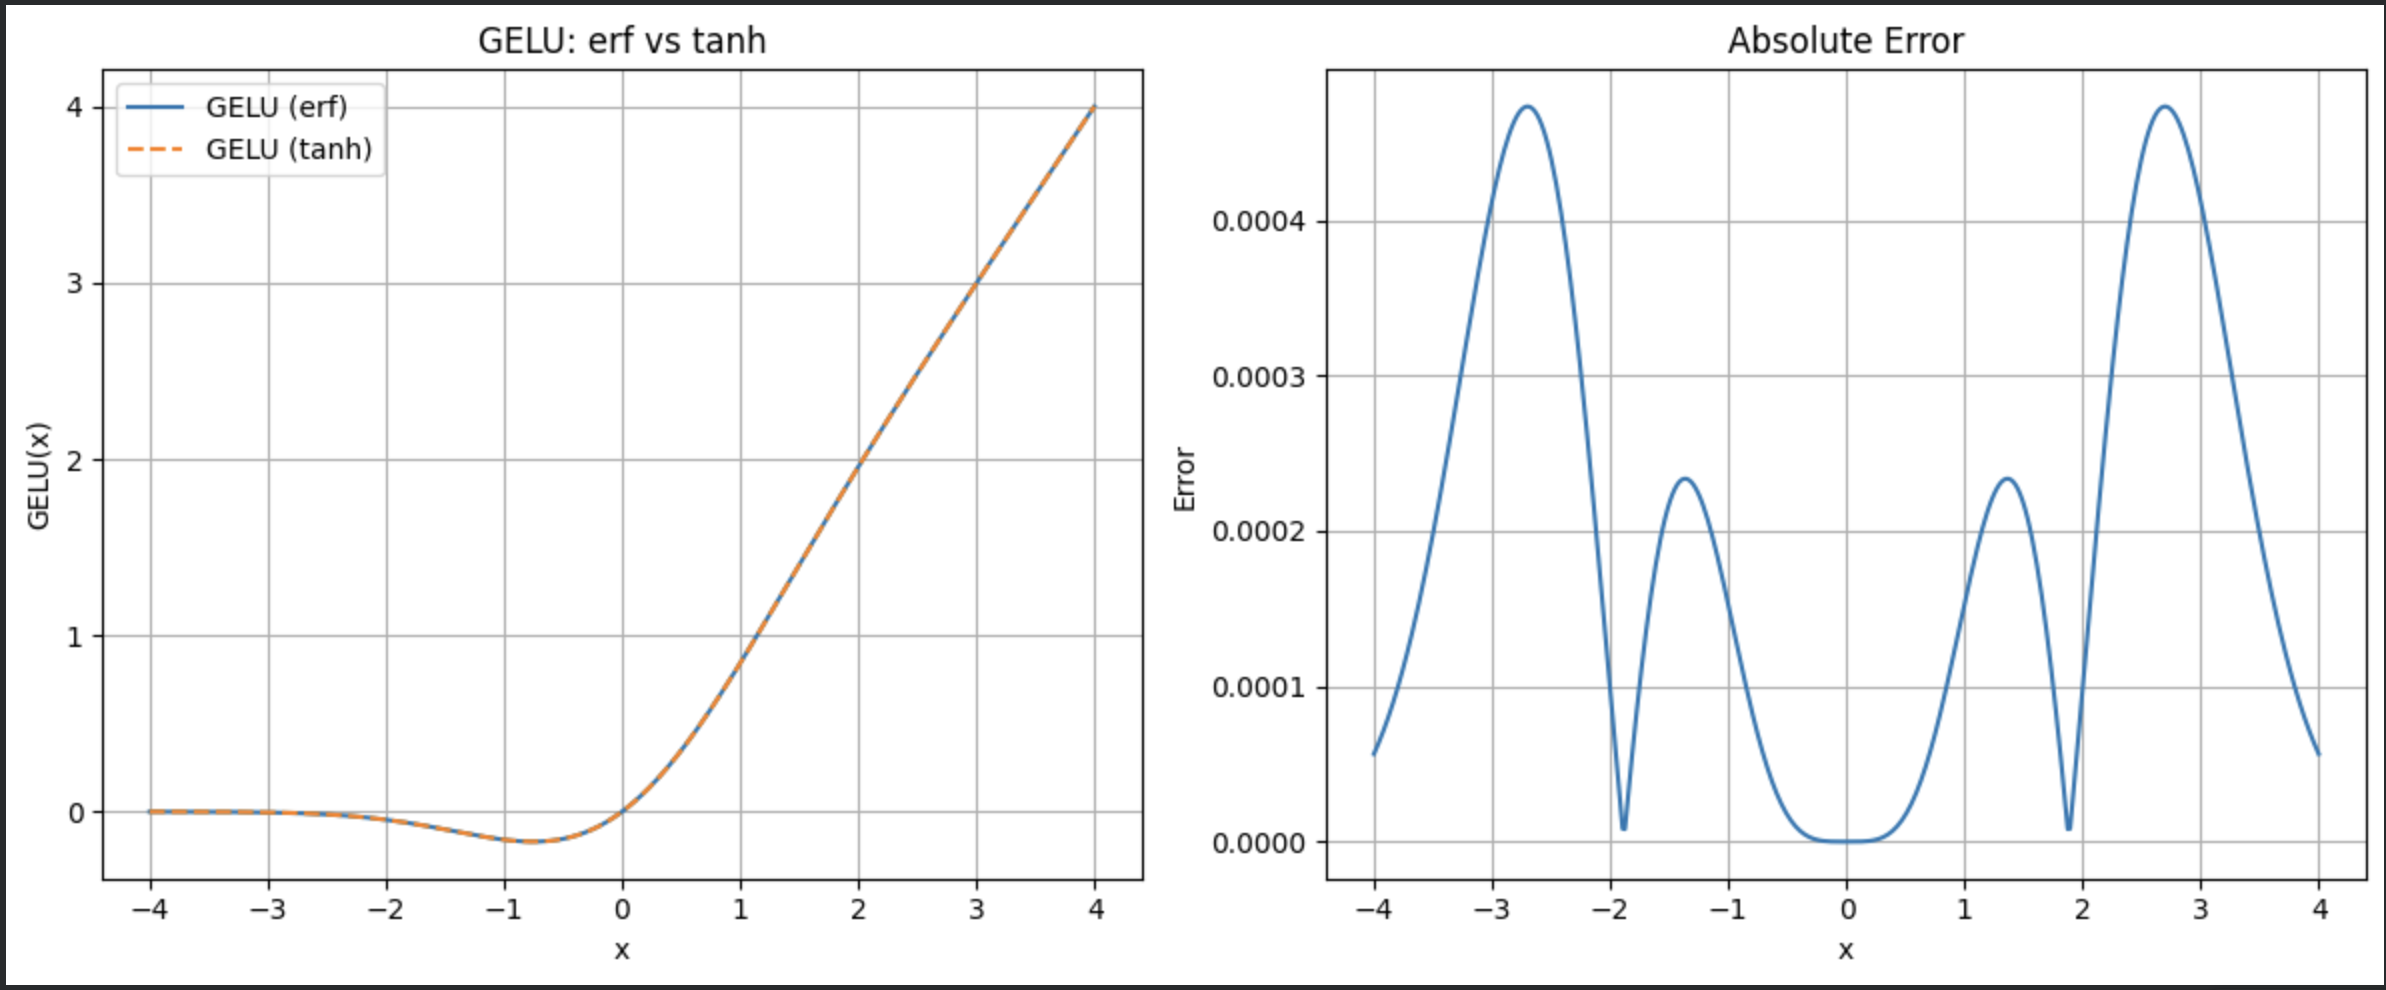
\includegraphics[width=0.8\textwidth]{images/gelu_approximation.png}
    \caption{Original GELU vs approximation}
    \label{fig:gelu_approx}
\end{figure}

\section{Synthesizable Softmax and Layer Normalization}

The other critical math functions in the ViT model are \texttt{expf} (for softmax) and \texttt{sqrtf} (for layer normalization and attention scaling).

\subsection{Softmax}
The \texttt{softmax\_seq} function, which is essential for the attention mechanism, is defined as:
\
Our code implements this using \texttt{expf()}:
\begin{verbatim}
scores[i] = expf(scores[i] - maxv);
\end{verbatim}
For this to be synthesizable, the Vitis HLS compiler must import \texttt{hls\_math.h} library \cite{ref4}. This instantiates a dedicated, pipelined hardware core that computes the exponential function, allowing the softmax to be implemented in hardware.

\subsection{Layer Normalization and Attention}
Similarly, the \texttt{layer\_norm} and \texttt{mha\_block} functions use \texttt{sqrtf()} to calculate the inverse square root of the variance and the attention scaling factor.
\begin{verbatim}
// In layer_norm
float inv = 1.0f / sqrtf(var + 1e-5f);

// In mha_block
const float inv_scale = 1.0f / sqrtf((float)HEAD_DIM);
\end{verbatim}
Just Like \texttt{expf}, these calls to \texttt{sqrtf} are also synthesizable by mapping them to the  \texttt{hls::sqrtf} function from the HLS math library \cite{ref4, ref5}.

\section{Conclusion: The Accuracy vs. Resource Trade-off}

The approximations used in this project are a fundamental component of the algorithm-hardware codesign. By replacing non-synthesizable software functions with hardware-friendly equivalents, we make the ViT algorithm implementable on an FPGA.

This introduces a critical trade-off between accuracy and resource cost \cite{ref7}. While the 32-bit floating-point approximations used in this project (like the GELU-tanh) are extremely accurate, they are resource-intensive. Each call to \texttt{hls::expf} or \texttt{hls::sqrtf} instantiates a complex hardware IP core that consumes FPGA logic and DSPs.

A more aggressive optimization, often used in resource-constrained edge devices, would be to replace these with 8-bit fixed-point polynomial or piecewise-linear approximations \cite{ref4, ref5}. However, the chosen approach (synthesizable \texttt{float}) represents a robust balance, prioritizing high numerical accuracy while still achieving the massive parallelism and acceleration offered by the FPGA.

\begin{table}[h!]
    \centering
    \begin{tabular}{|l|l|l|}
        \hline
        \textbf{Function} & \textbf{Original (Software)} & \textbf{HLS-Synthesizable Implementation} \\
        \hline
        \textbf{GELU} & Uses \texttt{erf()} & $\tanh$ approximation (as coded) \cite{ref6} \\
        \hline
        \textbf{Softmax} & Uses \texttt{expf()} from \texttt{math.h} & \texttt{hls::expf} from \texttt{hls\_math.h} \cite{ref4} \\
        \hline
        \textbf{Layer Norm} & Uses \texttt{sqrtf()} from \texttt{math.h} & \texttt{hls::sqrtf} from \texttt{hls\_math.h} \cite{ref4, ref5} \\
        \hline
        \textbf{Attention Scale} & Uses \texttt{sqrtf()} from \texttt{math.h} & \texttt{hls::sqrtf} from \texttt{hls\_math.h} \cite{ref4, ref5} \\
        \hline
    \end{tabular}
    \caption{Summary of mathematical functions and their HLS-synthesizable approximations.}
    \label{table:approx_summary}
\end{table}